\section{Reshaping data: wide to long and long to wide}\label{sec:pivot}

Data that you find or create does not always have the shape that you need it to be in for your analysis.
In many cases, for further data wrangling or for analyses you want each observation to be in its own row.
However, many data sources list multiple observations in columns.
For example, data from panel surveys asking the same question every week will often have one row per respondent,
and one column for each weekly measurement.
For a time-series analysis, however, each row should be a single measurement,
i.e. the unit of analysis is a respondent per week.

Generally, data with multiple observations of the same unit is called \concept{wide data} (as there are many column),
while a data set with one row for each observation is called \concept{long data} (as there are many rows).
In most cases, long data is easiest to work with, and in fact in \tidyverse\ jargon such data is called \concept[tidy data]{tidy}.

As a first relatively simple example, consider the data sets containing public and private capital.
This data is `wide' in the sense that the measurements for the different countries are contained in the columns.
To make this data `long' we would have to create rows for each country-year combination.
This will make it much easier to do further data wrangling or analysis, as you can now e.g. directly merge the data sets and compute the pooled correlation between these variables. 
In fact, when we merged these data sets earlier in \refex{merge}, we selected only the measurements for France, essentially turning it into long data.

\begin{ccsexample}
  \doublecodex{ch_data_wrangling/merge1}
  \codexoutputtable{ch_data_wrangling/merge1.r}
  \doublecodex{ch_data_wrangling/merge2}
  \codexoutputpng{ch_data_wrangling/merge2.r}
  \caption{Converting wide to long data to facilitate merging and visualizing}\label{ex:merge}
\end{ccsexample}

\refex{pivot} shows how you can `pivot' the capital data to long format using \fn{pivot\_longer} (R) and \fn{wide\_to\_long} (Pandas). The seccond part of this example then goes on to do this for both data sets, merge them, and partially reproduce Figure~4.4 from \citet{piketty}.

\section{Restructuring `messy' data}

As a final example, we will look at the data on income and wage shares from Piketty (supplemental tables S8.1 and S8.2).
We want to visualize the income and wage share going to the top 1\% earners in France and the U.S..
\reffig{messy} shows a screenshot of this data in Open Office, with the U.S. data having a similar shape.
For the previous examples, we used a clean csv version of this data, but now we will tackle the additional challenge
of dealing with the excel file including extra header rows and column names aimed at human consumption rather than easy computing. 

\begin{figure}
  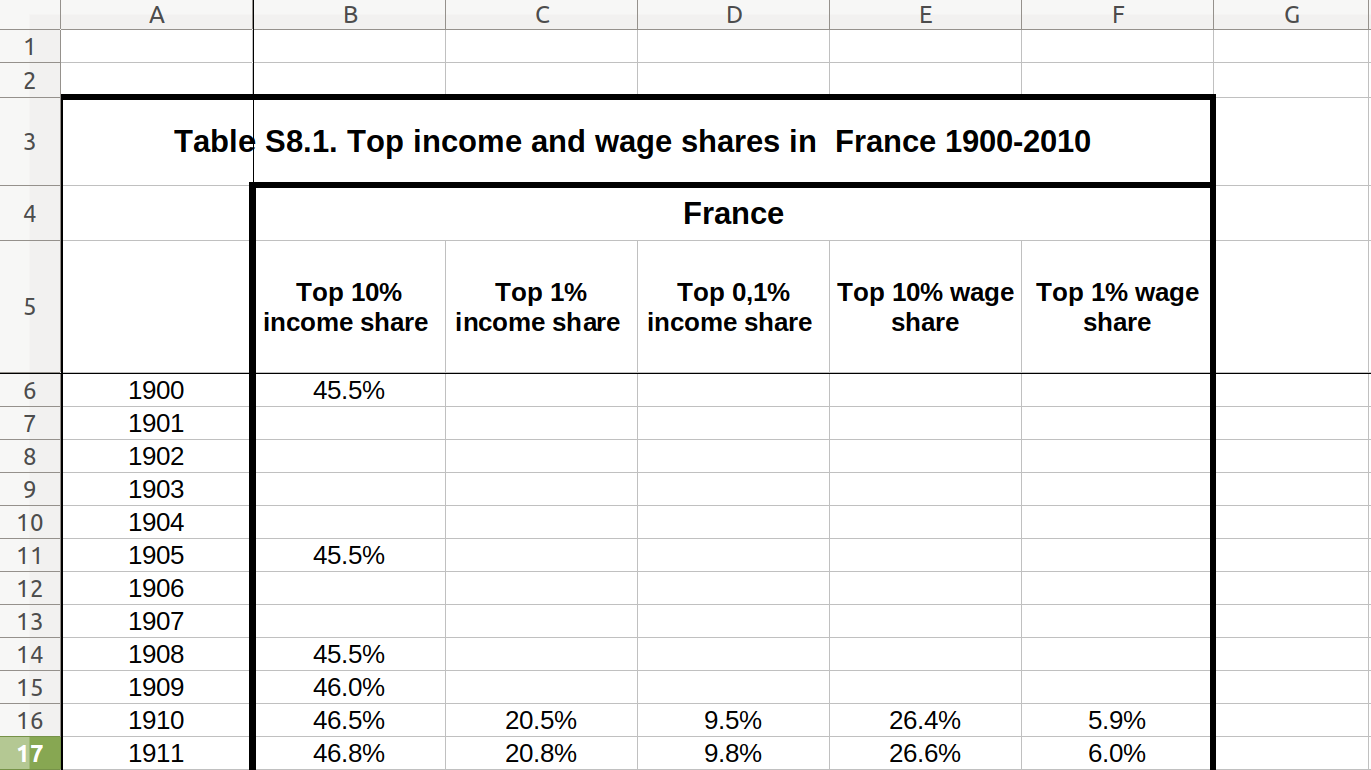
\includegraphics[width=\linewidth]{ch_data_wrangling/messy.png}
  \caption{Data on top incomes as provided in Piketty (2014; digital appendix)}\label{fig:messy}
\end{figure}

In order to perform our visualization, we want a data set containing a single measurement column (percentage share),
and a row for each year-country-type combination, i.e. one row for wage inequality in 1910 in the U.S..
One of the most important skills in computational social science (and data-driven analysis in general) is
understanding which series of generally small steps are needed to go from one data format to the other.
Although there is not a fixed step of steps that are always needed, the steps to get from the raw data visualized in \reffig{messy} to a `tidy' data set are fairly typical:

\begin{enumerate}
  \item Input: Read the data into data frames. In this case, reading from an excel sheet and skipping the extra header rows
  \item Reshape: Pivoting the data into long format
  \item Normalize: Normalize names, value types, etc. In this case, also separate a header like ``Top 1\% income share'' into income type (income, wage) and percentile (10\%, 1\%, etc)
  \item Filter: Filter for the desired data
  \item Analyze: Create the visualization
\end{enumerate}

Fortunately, These steps have been discussed before: reading csv data in \refsec{readdata}; pivot to long data in \refsec{pivot};
add a column in \refsec{calculate}; joining data in \refsec{join}; and visualizing in \refchap{visualize}.

\refex{excel} shows how to perform the first three steps for the U.S. case.
First, we use the \pkg{readxl} (R) and \pkg{xlrd} (Python) to read a sheet from an excel file into a data frame,
manually specifying the number of header and footer rows to skip.
Then, we pivot the columns into a
The missing step, splitting a header into two columns, is done using \fn{separate} (R) and \fn{split} (Python). 

\begin{ccsexample}
  \doublecodex{ch_data_wrangling/excel1}
  \codexoutputtable{ch_data_wrangling/excel1.r}
  \doublecodex{ch_data_wrangling/excel2}
  \codexoutputpng{ch_data_wrangling/excel2.py}
  \caption{Dealing with `messy' data}\label{ex:excel}
\end{ccsexample}
